\chapter{Numerical Results for the Asset Allocation Problem}

\section{Single Risky Asset Case}


\subsection{Simulated Data}
To test the different reinforcement learning methods in a controlled environment, we generated log price series as random walks with autoregressive trend processes. The two-
parameter model is thus given by
\begin{equation*}
	\begin{split}
		z_t &= z_{t-1} + \beta_{t-1} + \kappa \epsilon_t\\
		\beta_t &= \alpha \beta_{t-1} + \nu_t\\
	\end{split}
\end{equation*}
We then define the synthetic price series as
\begin{equation*}
	Z_t = \exp\left(\frac{z_t}{\max_t z_t - \min_t z_t}\right)
\end{equation*}
This process presents some patterns that can be profitably exploited and therefore we would expect our learning algorithms to perform well on this test case. In the following subsections we will compare the results of three long-short strategies obtained with ARAC, PGPE and NPGPE in both the risk-neutral and risk-sensitive framework. Let us describe the choice we made for each of the algorithms. 

\subsubsection{ARAC} 
For the ARAC algorithm we considered a Boltzmann exploration policy on the two actions $a_t^1 \in \{-1, 1\}$ and a linear critic. This critic is extremely simple and there is surely some work to be done to improve it. 

\subsubsection{PGPE}
For the PGPE algorithm we considered a binary deterministic controller 
\begin{equation*}
	F_\theta(s) = \sign(\theta \cdot s)
\end{equation*}
where the parameters and the state also include a bias term. The controller parameters are sampled from a multi-variate Gaussian distribution
\begin{equation*}
	\theta \sim \calN(\mu, \diag(\sigma))
\end{equation*}  

\subsubsection{NPGPE}
In NPGPE, we used the same controller as for PGPE but we assumed that the controller parameters are sampled from a Gaussian distribution parameterized by its mean and Cholesky factor
\begin{equation*}
	\theta \sim \calN(\mu, C^T C)
\end{equation*}  


\subsubsection{Experimental Setup}   
All the algorithms were tested on the same price series of size $10000$, generated from the process described above using $\alpha = 0.9$ and $\kappa = 3$. The learning process consisted of $500$ training epochs on the first $7500$ days of the series with a learning rate that decreased at each epoch according to a polynomial schedule. The trained agents were subsequently backtested on the final $2500$ days, during which the agents kept learning online in order to try to adapt to the changing environment. The results that we present are the average of $10$ independent experiments that used slightly different random initialization of the policy parameters.   

\subsubsection{Results}

\begin{figure}[t]
	\centering
	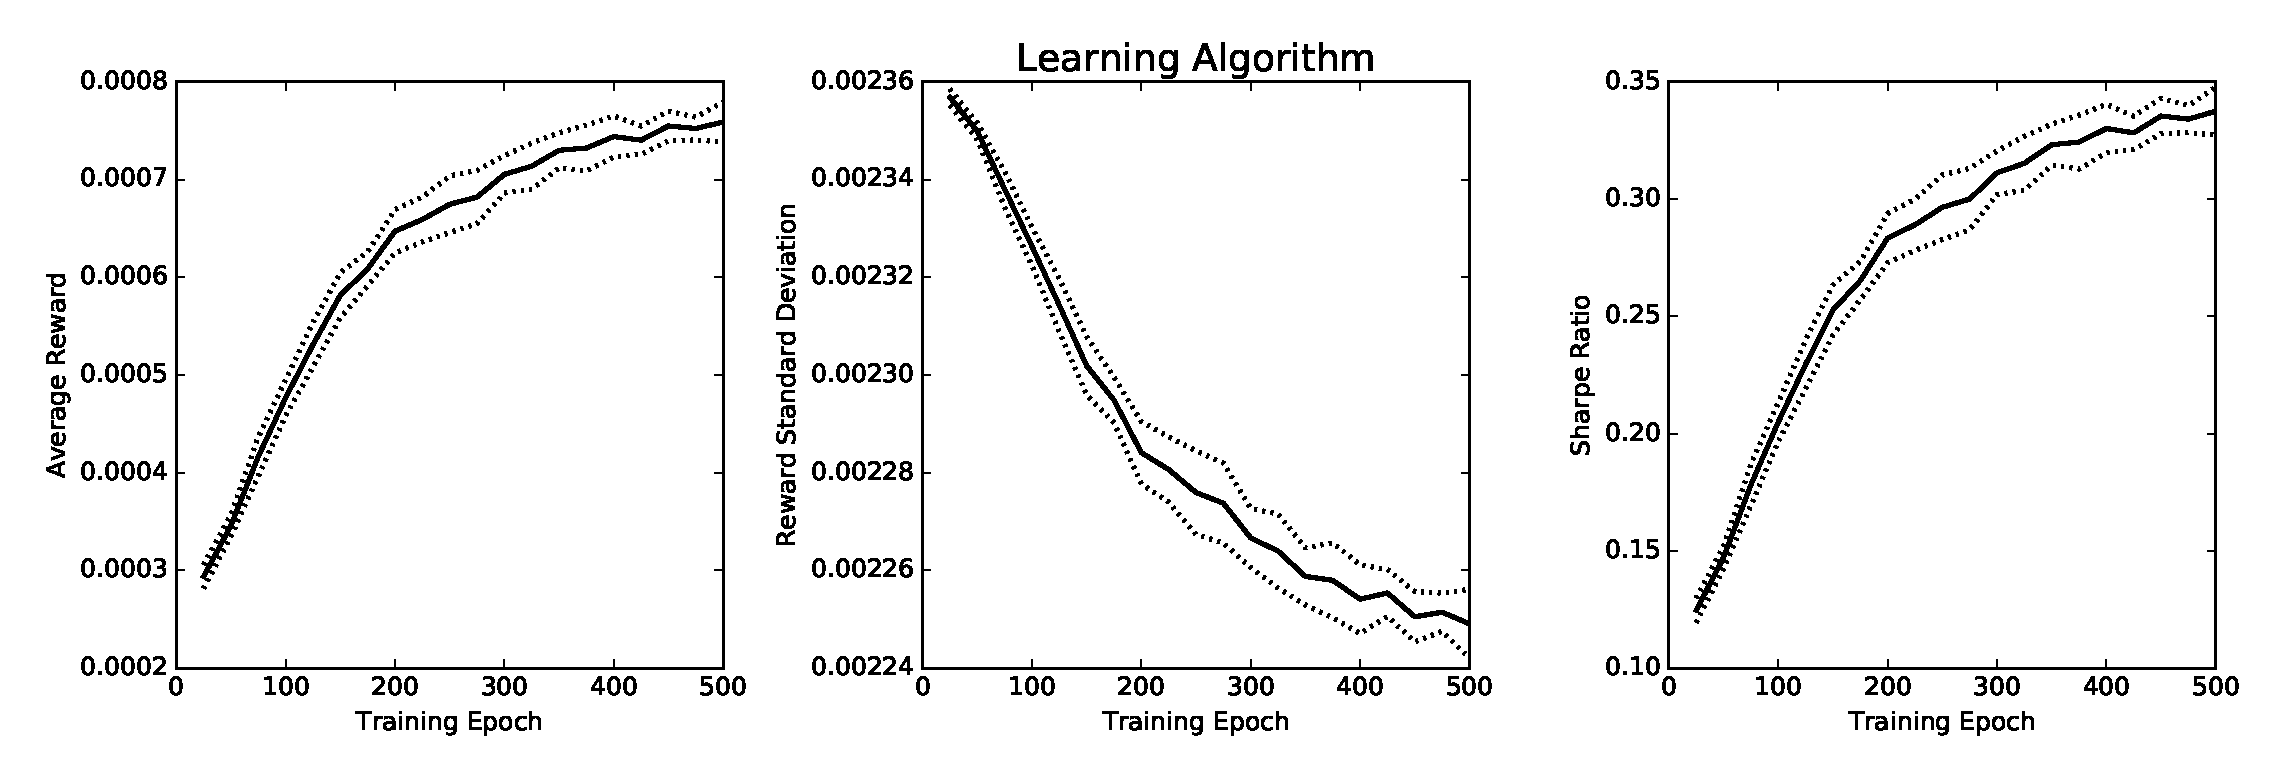
\includegraphics[width=1.0\textwidth]{Images/6_0_single_synthetic_convergence}
	\caption[Learning process for one synthetic risky asset]{Learning process for the asset allocation problem with one synthetic risky asset.}
	\label{fig:single_synthetic_convergence}
\end{figure}

\begin{figure}[t]
	\centering
	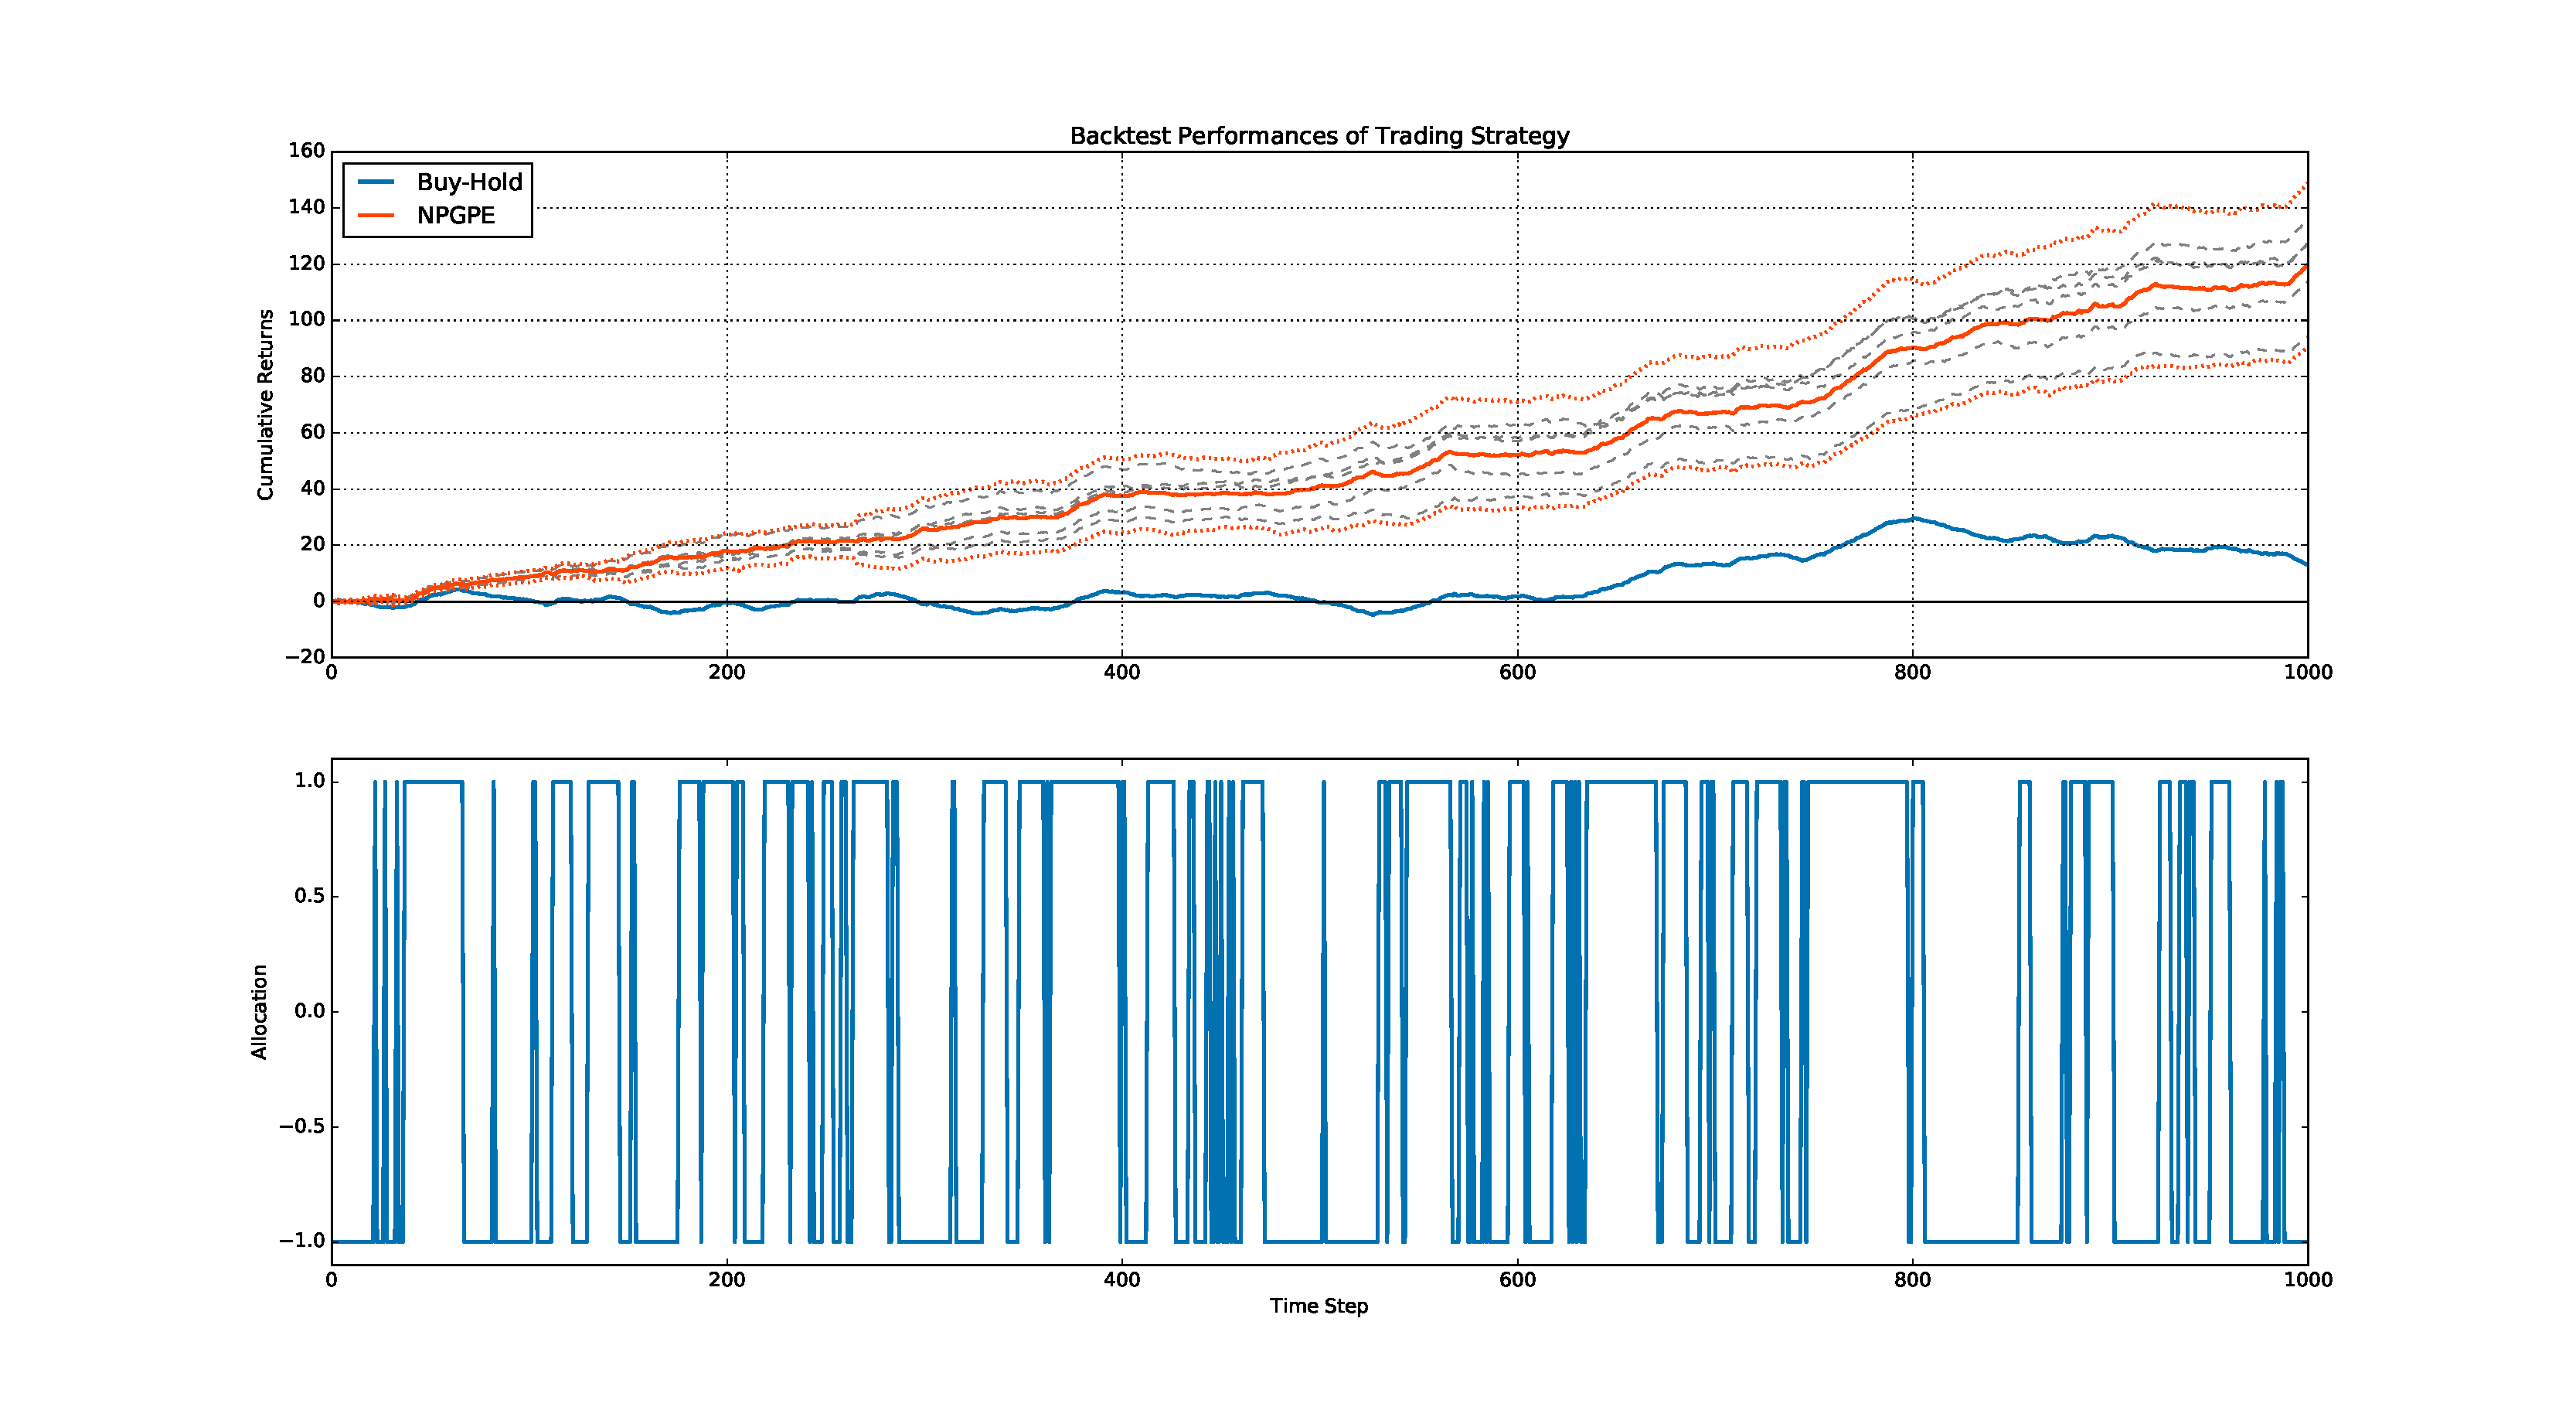
\includegraphics[width=1.0\textwidth]{Images/6_1_single_synthetic_performance}
	\caption[Backtest performance with one synthetic risky asset]{Backtest performance of trained trading systems for the asset allocation problem with one synthetic risky asset.}
	\label{fig:single_synthetic_performance}
\end{figure}

\begin{figure}[t]
	\centering
	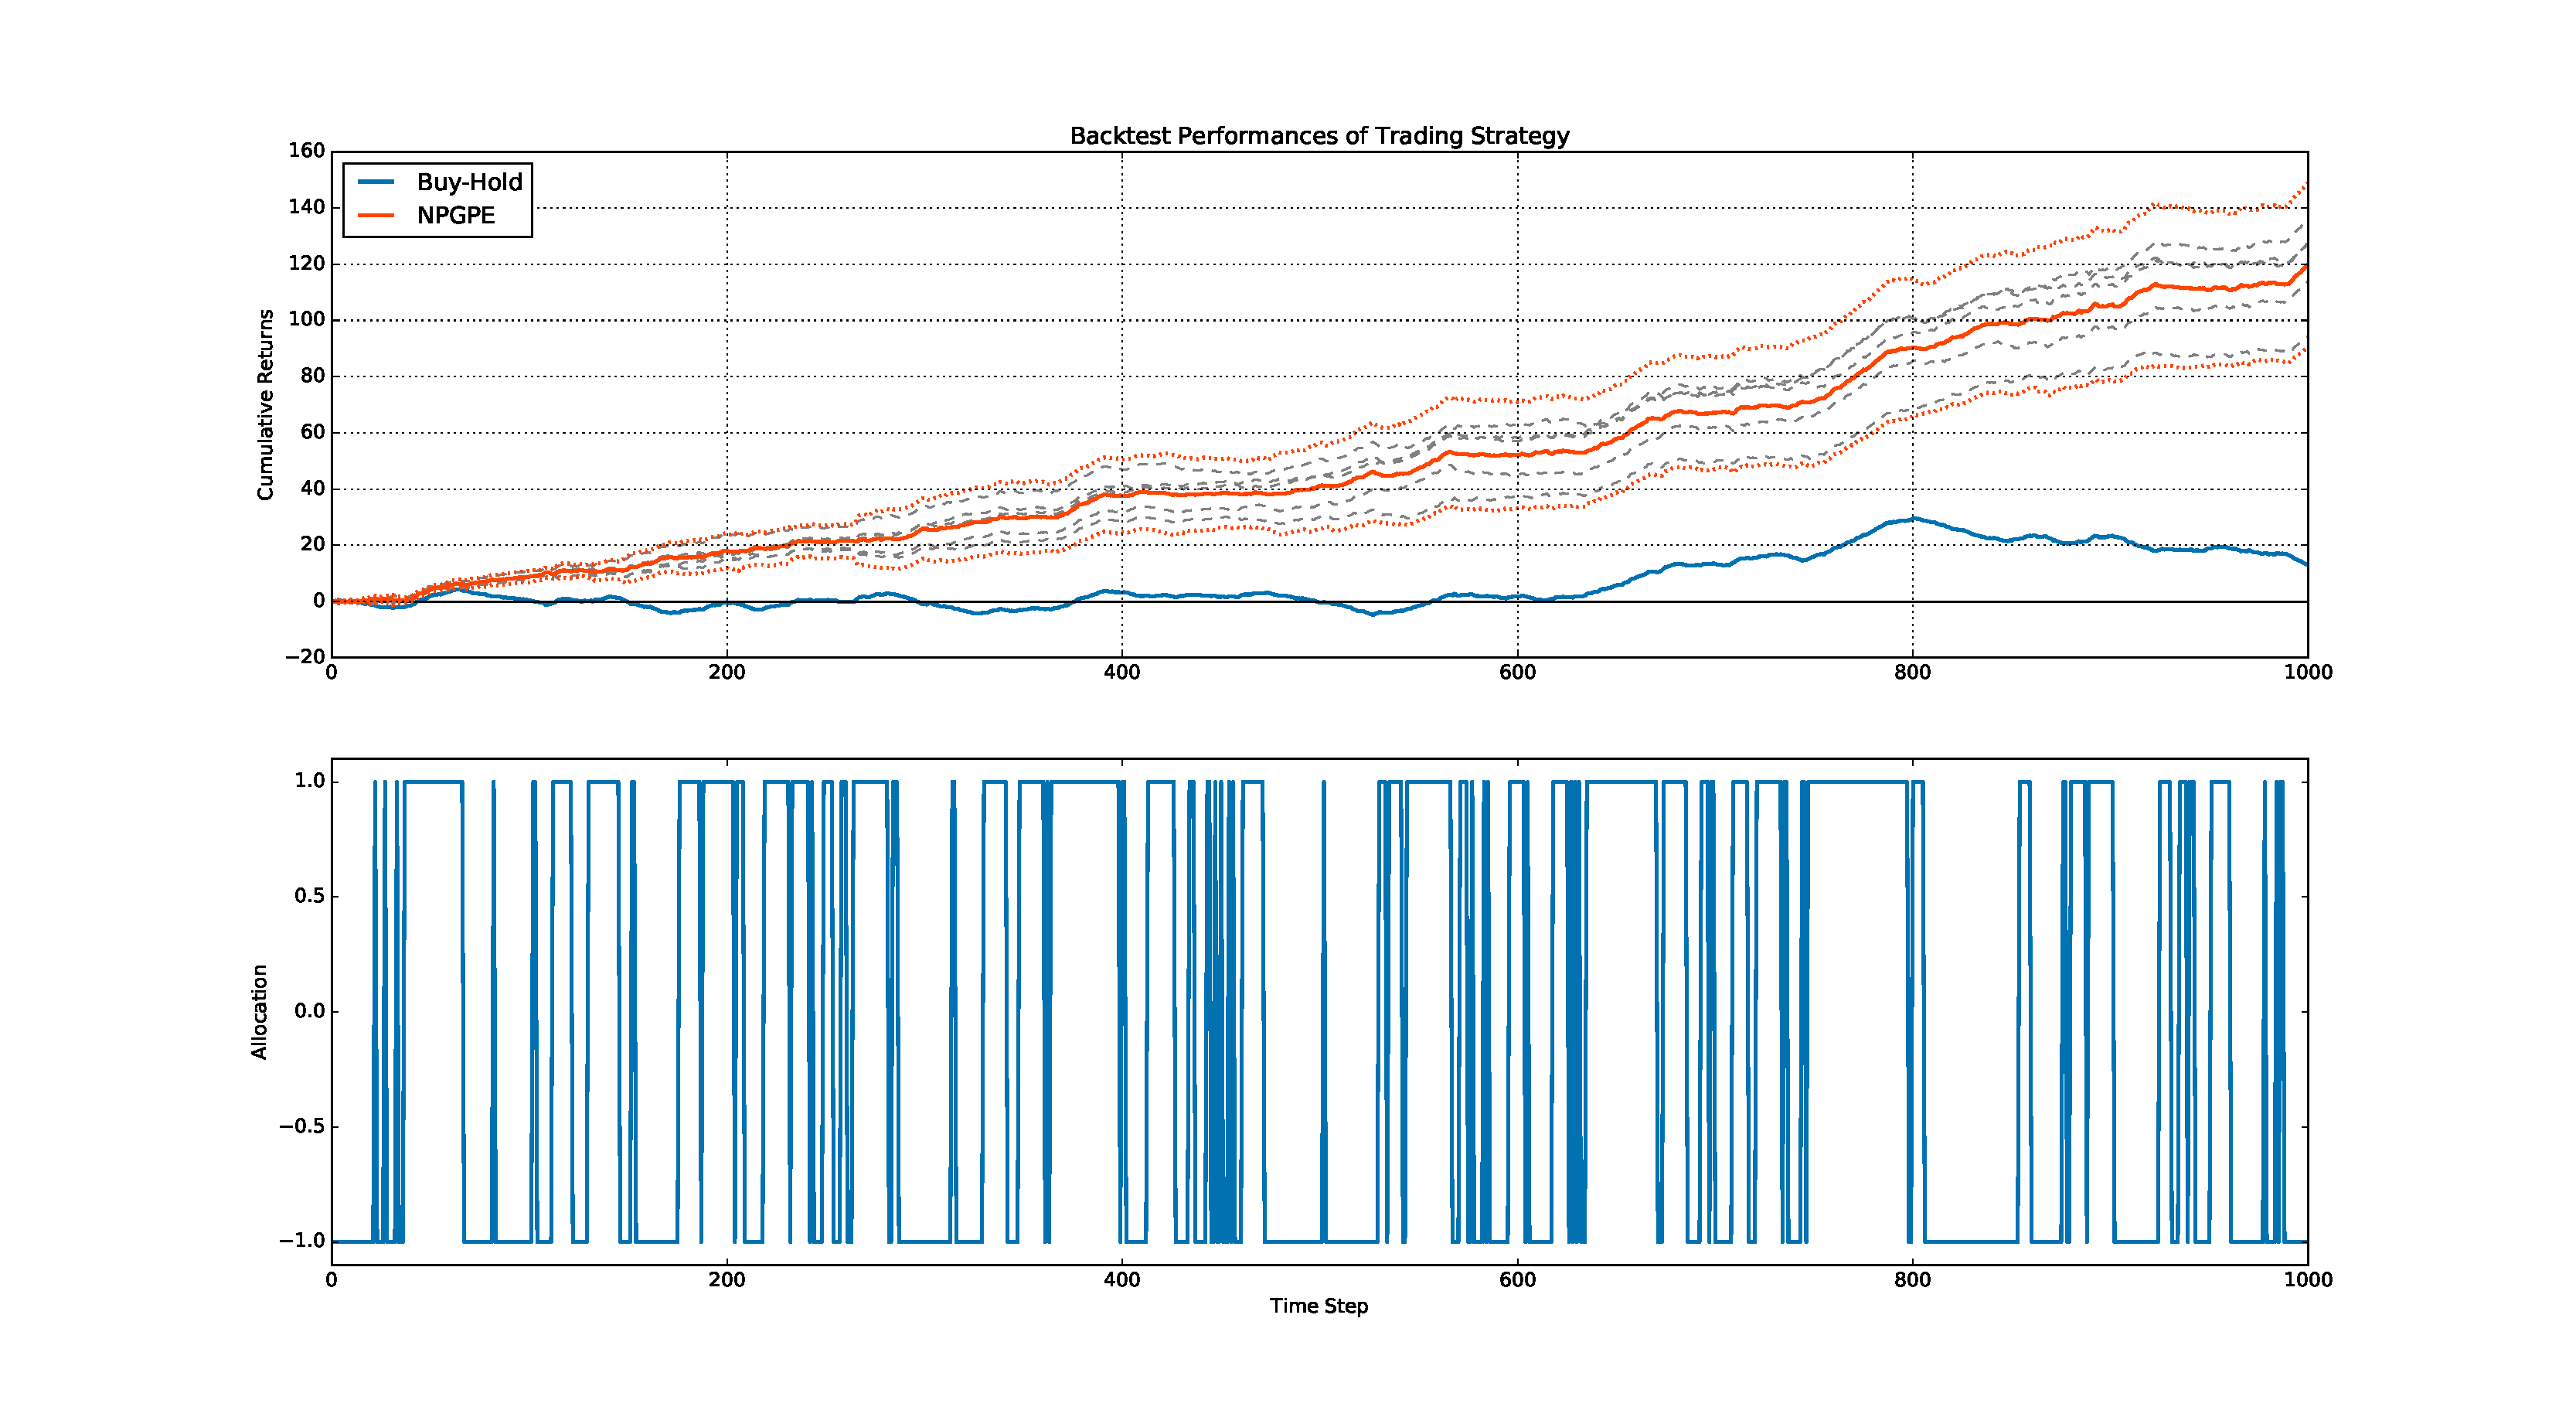
\includegraphics[width=1.0\textwidth]{Images/6_2_single_synthetic_NPGPE}
	\caption[Backtest performance of NPGPE with one synthetic risky asset]{Backtest performance and allocation selected by the NPGPE algorithm for the asset allocation problem with one synthetic risky asset.}
	\label{fig:single_synthetic_NPGPE}
\end{figure}

%TODO: Reallocation frequence as a function of transaction costs
%TODO: Comparative table with backtest statistics

\subsection{Historic Data}



\section{Multiple Risky Asset Case}

\subsection{Simulated Data}


\subsection{Historic Data}